% Created by tikzDevice version 0.11 on 2018-03-25 11:03:35
% !TEX encoding = UTF-8 Unicode
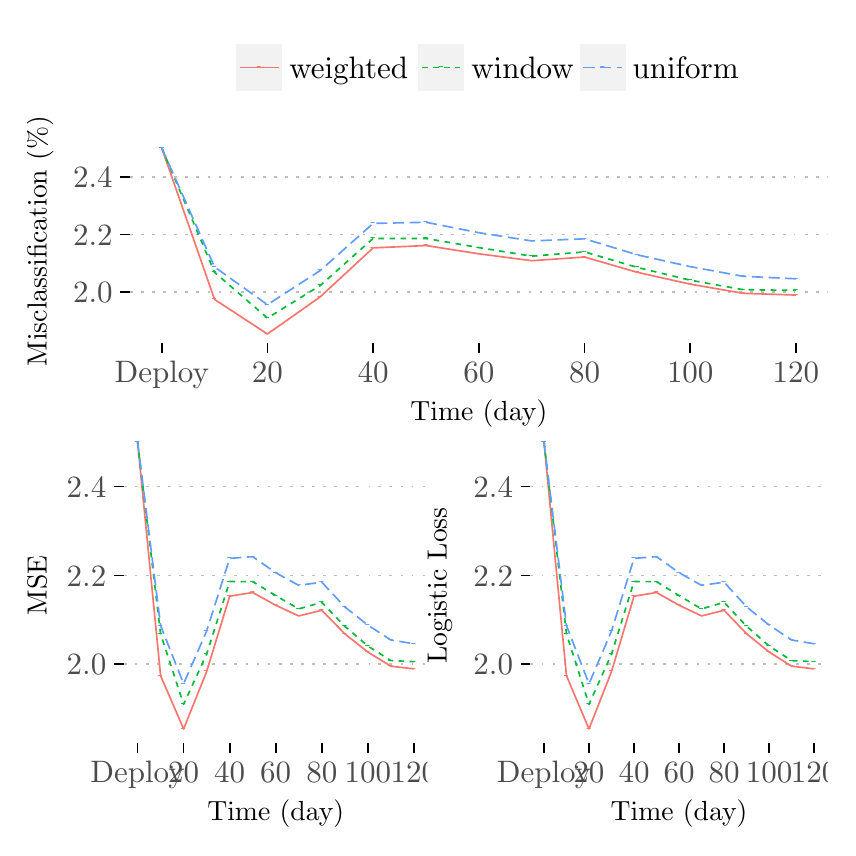
\begin{tikzpicture}[x=1pt,y=1pt]
\definecolor{fillColor}{RGB}{255,255,255}
\path[use as bounding box,fill=fillColor,fill opacity=0.00] (0,0) rectangle (289.08,289.08);
\begin{scope}
\path[clip] (  0.00,144.54) rectangle (289.08,289.08);
\definecolor{drawColor}{RGB}{255,255,255}
\definecolor{fillColor}{RGB}{255,255,255}

\path[draw=drawColor,line width= 0.6pt,line join=round,line cap=round,fill=fillColor] (  0.00,144.54) rectangle (289.08,289.08);
\end{scope}
\begin{scope}
\path[clip] ( 36.99,175.02) rectangle (289.08,248.97);
\definecolor{fillColor}{RGB}{255,255,255}

\path[fill=fillColor] ( 36.99,175.02) rectangle (289.08,248.97);
\definecolor{drawColor}{RGB}{255,255,255}

\path[draw=drawColor,line width= 0.3pt,line join=round] ( 36.99,183.12) --
	(289.08,183.12);

\path[draw=drawColor,line width= 0.3pt,line join=round] ( 36.99,203.95) --
	(289.08,203.95);

\path[draw=drawColor,line width= 0.3pt,line join=round] ( 36.99,224.78) --
	(289.08,224.78);

\path[draw=drawColor,line width= 0.3pt,line join=round] ( 36.99,245.61) --
	(289.08,245.61);

\path[draw=drawColor,line width= 0.3pt,line join=round] ( 67.54,175.02) --
	( 67.54,248.97);

\path[draw=drawColor,line width= 0.3pt,line join=round] (105.73,175.02) --
	(105.73,248.97);

\path[draw=drawColor,line width= 0.3pt,line join=round] (143.93,175.02) --
	(143.93,248.97);

\path[draw=drawColor,line width= 0.3pt,line join=round] (182.12,175.02) --
	(182.12,248.97);

\path[draw=drawColor,line width= 0.3pt,line join=round] (220.32,175.02) --
	(220.32,248.97);

\path[draw=drawColor,line width= 0.3pt,line join=round] (258.52,175.02) --
	(258.52,248.97);
\definecolor{drawColor}{RGB}{190,190,190}

\path[draw=drawColor,line width= 0.6pt,dash pattern=on 1pt off 3pt ,line join=round] ( 36.99,193.53) --
	(289.08,193.53);

\path[draw=drawColor,line width= 0.6pt,dash pattern=on 1pt off 3pt ,line join=round] ( 36.99,214.37) --
	(289.08,214.37);

\path[draw=drawColor,line width= 0.6pt,dash pattern=on 1pt off 3pt ,line join=round] ( 36.99,235.20) --
	(289.08,235.20);
\definecolor{drawColor}{RGB}{255,255,255}

\path[draw=drawColor,line width= 0.6pt,line join=round] ( 48.45,175.02) --
	( 48.45,248.97);

\path[draw=drawColor,line width= 0.6pt,line join=round] ( 86.63,175.02) --
	( 86.63,248.97);

\path[draw=drawColor,line width= 0.6pt,line join=round] (124.83,175.02) --
	(124.83,248.97);

\path[draw=drawColor,line width= 0.6pt,line join=round] (163.02,175.02) --
	(163.02,248.97);

\path[draw=drawColor,line width= 0.6pt,line join=round] (201.22,175.02) --
	(201.22,248.97);

\path[draw=drawColor,line width= 0.6pt,line join=round] (239.42,175.02) --
	(239.42,248.97);

\path[draw=drawColor,line width= 0.6pt,line join=round] (277.62,175.02) --
	(277.62,248.97);
\definecolor{drawColor}{RGB}{248,118,109}

\path[draw=drawColor,line width= 0.6pt,line join=round] ( 48.45,245.61) --
	( 67.53,190.88) --
	( 86.63,178.38) --
	(105.73,191.83) --
	(124.83,209.50) --
	(143.93,210.35) --
	(163.02,207.37) --
	(182.12,204.87) --
	(201.22,206.19) --
	(220.32,200.67) --
	(239.42,196.40) --
	(258.52,193.09) --
	(277.62,192.46);
\definecolor{drawColor}{RGB}{0,186,56}

\path[draw=drawColor,line width= 0.6pt,dash pattern=on 2pt off 2pt ,line join=round] ( 48.45,245.61) --
	( 67.53,200.67) --
	( 86.63,184.16) --
	(105.73,195.91) --
	(124.83,212.92) --
	(143.93,212.90) --
	(163.02,209.62) --
	(182.12,206.51) --
	(201.22,208.05) --
	(220.32,202.44) --
	(239.42,197.83) --
	(258.52,194.40) --
	(277.62,194.15);
\definecolor{drawColor}{RGB}{97,156,255}

\path[draw=drawColor,line width= 0.6pt,dash pattern=on 4pt off 2pt ,line join=round] ( 48.45,245.61) --
	( 67.53,202.60) --
	( 86.63,188.98) --
	(105.73,201.33) --
	(124.83,218.35) --
	(143.93,218.76) --
	(163.02,214.99) --
	(182.12,212.02) --
	(201.22,212.78) --
	(220.32,206.98) --
	(239.42,202.73) --
	(258.52,199.23) --
	(277.62,198.34);
\definecolor{drawColor}{RGB}{248,118,109}

\node[text=drawColor,anchor=base,inner sep=0pt, outer sep=0pt, scale=  0.58] at ( 48.45,244.37) {-};

\node[text=drawColor,anchor=base,inner sep=0pt, outer sep=0pt, scale=  0.58] at ( 67.53,189.63) {-};

\node[text=drawColor,anchor=base,inner sep=0pt, outer sep=0pt, scale=  0.58] at ( 86.63,177.14) {-};

\node[text=drawColor,anchor=base,inner sep=0pt, outer sep=0pt, scale=  0.58] at (105.73,190.59) {-};

\node[text=drawColor,anchor=base,inner sep=0pt, outer sep=0pt, scale=  0.58] at (124.83,208.25) {-};

\node[text=drawColor,anchor=base,inner sep=0pt, outer sep=0pt, scale=  0.58] at (143.93,209.11) {-};

\node[text=drawColor,anchor=base,inner sep=0pt, outer sep=0pt, scale=  0.58] at (163.02,206.12) {-};

\node[text=drawColor,anchor=base,inner sep=0pt, outer sep=0pt, scale=  0.58] at (182.12,203.62) {-};

\node[text=drawColor,anchor=base,inner sep=0pt, outer sep=0pt, scale=  0.58] at (201.22,204.95) {-};

\node[text=drawColor,anchor=base,inner sep=0pt, outer sep=0pt, scale=  0.58] at (220.32,199.43) {-};

\node[text=drawColor,anchor=base,inner sep=0pt, outer sep=0pt, scale=  0.58] at (239.42,195.16) {-};

\node[text=drawColor,anchor=base,inner sep=0pt, outer sep=0pt, scale=  0.58] at (258.52,191.84) {-};

\node[text=drawColor,anchor=base,inner sep=0pt, outer sep=0pt, scale=  0.58] at (277.62,191.22) {-};
\definecolor{drawColor}{RGB}{0,186,56}

\node[text=drawColor,anchor=base,inner sep=0pt, outer sep=0pt, scale=  0.58] at ( 48.45,244.37) {-};

\node[text=drawColor,anchor=base,inner sep=0pt, outer sep=0pt, scale=  0.58] at ( 67.53,199.42) {-};

\node[text=drawColor,anchor=base,inner sep=0pt, outer sep=0pt, scale=  0.58] at ( 86.63,182.92) {-};

\node[text=drawColor,anchor=base,inner sep=0pt, outer sep=0pt, scale=  0.58] at (105.73,194.67) {-};

\node[text=drawColor,anchor=base,inner sep=0pt, outer sep=0pt, scale=  0.58] at (124.83,211.68) {-};

\node[text=drawColor,anchor=base,inner sep=0pt, outer sep=0pt, scale=  0.58] at (143.93,211.66) {-};

\node[text=drawColor,anchor=base,inner sep=0pt, outer sep=0pt, scale=  0.58] at (163.02,208.37) {-};

\node[text=drawColor,anchor=base,inner sep=0pt, outer sep=0pt, scale=  0.58] at (182.12,205.27) {-};

\node[text=drawColor,anchor=base,inner sep=0pt, outer sep=0pt, scale=  0.58] at (201.22,206.81) {-};

\node[text=drawColor,anchor=base,inner sep=0pt, outer sep=0pt, scale=  0.58] at (220.32,201.20) {-};

\node[text=drawColor,anchor=base,inner sep=0pt, outer sep=0pt, scale=  0.58] at (239.42,196.58) {-};

\node[text=drawColor,anchor=base,inner sep=0pt, outer sep=0pt, scale=  0.58] at (258.52,193.15) {-};

\node[text=drawColor,anchor=base,inner sep=0pt, outer sep=0pt, scale=  0.58] at (277.62,192.90) {-};
\definecolor{drawColor}{RGB}{97,156,255}

\node[text=drawColor,anchor=base,inner sep=0pt, outer sep=0pt, scale=  0.58] at ( 48.45,244.37) {-};

\node[text=drawColor,anchor=base,inner sep=0pt, outer sep=0pt, scale=  0.58] at ( 67.53,201.35) {-};

\node[text=drawColor,anchor=base,inner sep=0pt, outer sep=0pt, scale=  0.58] at ( 86.63,187.73) {-};

\node[text=drawColor,anchor=base,inner sep=0pt, outer sep=0pt, scale=  0.58] at (105.73,200.08) {-};

\node[text=drawColor,anchor=base,inner sep=0pt, outer sep=0pt, scale=  0.58] at (124.83,217.10) {-};

\node[text=drawColor,anchor=base,inner sep=0pt, outer sep=0pt, scale=  0.58] at (143.93,217.51) {-};

\node[text=drawColor,anchor=base,inner sep=0pt, outer sep=0pt, scale=  0.58] at (163.02,213.75) {-};

\node[text=drawColor,anchor=base,inner sep=0pt, outer sep=0pt, scale=  0.58] at (182.12,210.77) {-};

\node[text=drawColor,anchor=base,inner sep=0pt, outer sep=0pt, scale=  0.58] at (201.22,211.53) {-};

\node[text=drawColor,anchor=base,inner sep=0pt, outer sep=0pt, scale=  0.58] at (220.32,205.74) {-};

\node[text=drawColor,anchor=base,inner sep=0pt, outer sep=0pt, scale=  0.58] at (239.42,201.48) {-};

\node[text=drawColor,anchor=base,inner sep=0pt, outer sep=0pt, scale=  0.58] at (258.52,197.98) {-};

\node[text=drawColor,anchor=base,inner sep=0pt, outer sep=0pt, scale=  0.58] at (277.62,197.10) {-};
\end{scope}
\begin{scope}
\path[clip] (  0.00,  0.00) rectangle (289.08,289.08);
\definecolor{drawColor}{gray}{0.30}

\node[text=drawColor,anchor=base east,inner sep=0pt, outer sep=0pt, scale=  1.12] at ( 30.69,189.68) {2.0};

\node[text=drawColor,anchor=base east,inner sep=0pt, outer sep=0pt, scale=  1.12] at ( 30.69,210.51) {2.2};

\node[text=drawColor,anchor=base east,inner sep=0pt, outer sep=0pt, scale=  1.12] at ( 30.69,231.34) {2.4};
\end{scope}
\begin{scope}
\path[clip] (  0.00,  0.00) rectangle (289.08,289.08);
\definecolor{drawColor}{RGB}{0,0,0}

\path[draw=drawColor,line width= 0.6pt,line join=round] ( 33.49,193.53) --
	( 36.99,193.53);

\path[draw=drawColor,line width= 0.6pt,line join=round] ( 33.49,214.37) --
	( 36.99,214.37);

\path[draw=drawColor,line width= 0.6pt,line join=round] ( 33.49,235.20) --
	( 36.99,235.20);
\end{scope}
\begin{scope}
\path[clip] (  0.00,  0.00) rectangle (289.08,289.08);
\definecolor{drawColor}{RGB}{0,0,0}

\path[draw=drawColor,line width= 0.6pt,line join=round] ( 48.45,171.52) --
	( 48.45,175.02);

\path[draw=drawColor,line width= 0.6pt,line join=round] ( 86.63,171.52) --
	( 86.63,175.02);

\path[draw=drawColor,line width= 0.6pt,line join=round] (124.83,171.52) --
	(124.83,175.02);

\path[draw=drawColor,line width= 0.6pt,line join=round] (163.02,171.52) --
	(163.02,175.02);

\path[draw=drawColor,line width= 0.6pt,line join=round] (201.22,171.52) --
	(201.22,175.02);

\path[draw=drawColor,line width= 0.6pt,line join=round] (239.42,171.52) --
	(239.42,175.02);

\path[draw=drawColor,line width= 0.6pt,line join=round] (277.62,171.52) --
	(277.62,175.02);
\end{scope}
\begin{scope}
\path[clip] (  0.00,  0.00) rectangle (289.08,289.08);
\definecolor{drawColor}{gray}{0.30}

\node[text=drawColor,anchor=base,inner sep=0pt, outer sep=0pt, scale=  1.12] at ( 48.45,161.00) {Deploy};

\node[text=drawColor,anchor=base,inner sep=0pt, outer sep=0pt, scale=  1.12] at ( 86.63,161.00) {20};

\node[text=drawColor,anchor=base,inner sep=0pt, outer sep=0pt, scale=  1.12] at (124.83,161.00) {40};

\node[text=drawColor,anchor=base,inner sep=0pt, outer sep=0pt, scale=  1.12] at (163.02,161.00) {60};

\node[text=drawColor,anchor=base,inner sep=0pt, outer sep=0pt, scale=  1.12] at (201.22,161.00) {80};

\node[text=drawColor,anchor=base,inner sep=0pt, outer sep=0pt, scale=  1.12] at (239.42,161.00) {100};

\node[text=drawColor,anchor=base,inner sep=0pt, outer sep=0pt, scale=  1.12] at (277.62,161.00) {120};
\end{scope}
\begin{scope}
\path[clip] (  0.00,  0.00) rectangle (289.08,289.08);
\definecolor{drawColor}{RGB}{0,0,0}

\node[text=drawColor,anchor=base,inner sep=0pt, outer sep=0pt, scale=  1.00] at (163.03,147.12) {Time (day)};
\end{scope}
\begin{scope}
\path[clip] (  0.00,  0.00) rectangle (289.08,289.08);
\definecolor{drawColor}{RGB}{0,0,0}

\node[text=drawColor,rotate= 90.00,anchor=base,inner sep=0pt, outer sep=0pt, scale=  1.00] at (  6.89,212.00) {Misclassification (\%)};
\end{scope}
\begin{scope}
\path[clip] (  0.00,  0.00) rectangle (289.08,289.08);
\definecolor{fillColor}{RGB}{255,255,255}

\path[fill=fillColor] ( 65.00,260.35) rectangle (261.07,289.08);
\end{scope}
\begin{scope}
\path[clip] (  0.00,  0.00) rectangle (289.08,289.08);
\definecolor{drawColor}{RGB}{255,255,255}
\definecolor{fillColor}{gray}{0.95}

\path[draw=drawColor,line width= 0.6pt,line join=round,line cap=round,fill=fillColor] ( 75.03,266.04) rectangle ( 92.37,283.39);
\end{scope}
\begin{scope}
\path[clip] (  0.00,  0.00) rectangle (289.08,289.08);
\definecolor{drawColor}{RGB}{248,118,109}

\path[draw=drawColor,line width= 0.6pt,line join=round] ( 76.76,274.72) -- ( 90.64,274.72);
\end{scope}
\begin{scope}
\path[clip] (  0.00,  0.00) rectangle (289.08,289.08);
\definecolor{drawColor}{RGB}{248,118,109}

\node[text=drawColor,anchor=base,inner sep=0pt, outer sep=0pt, scale=  0.58] at ( 83.70,273.47) {-};
\end{scope}
\begin{scope}
\path[clip] (  0.00,  0.00) rectangle (289.08,289.08);
\definecolor{drawColor}{RGB}{255,255,255}
\definecolor{fillColor}{gray}{0.95}

\path[draw=drawColor,line width= 0.6pt,line join=round,line cap=round,fill=fillColor] (140.78,266.04) rectangle (158.13,283.39);
\end{scope}
\begin{scope}
\path[clip] (  0.00,  0.00) rectangle (289.08,289.08);
\definecolor{drawColor}{RGB}{0,186,56}

\path[draw=drawColor,line width= 0.6pt,dash pattern=on 2pt off 2pt ,line join=round] (142.52,274.72) -- (156.39,274.72);
\end{scope}
\begin{scope}
\path[clip] (  0.00,  0.00) rectangle (289.08,289.08);
\definecolor{drawColor}{RGB}{0,186,56}

\node[text=drawColor,anchor=base,inner sep=0pt, outer sep=0pt, scale=  0.58] at (149.46,273.47) {-};
\end{scope}
\begin{scope}
\path[clip] (  0.00,  0.00) rectangle (289.08,289.08);
\definecolor{drawColor}{RGB}{255,255,255}
\definecolor{fillColor}{gray}{0.95}

\path[draw=drawColor,line width= 0.6pt,line join=round,line cap=round,fill=fillColor] (199.11,266.04) rectangle (216.45,283.39);
\end{scope}
\begin{scope}
\path[clip] (  0.00,  0.00) rectangle (289.08,289.08);
\definecolor{drawColor}{RGB}{97,156,255}

\path[draw=drawColor,line width= 0.6pt,dash pattern=on 4pt off 2pt ,line join=round] (200.84,274.72) -- (214.72,274.72);
\end{scope}
\begin{scope}
\path[clip] (  0.00,  0.00) rectangle (289.08,289.08);
\definecolor{drawColor}{RGB}{97,156,255}

\node[text=drawColor,anchor=base,inner sep=0pt, outer sep=0pt, scale=  0.58] at (207.78,273.47) {-};
\end{scope}
\begin{scope}
\path[clip] (  0.00,  0.00) rectangle (289.08,289.08);
\definecolor{drawColor}{RGB}{0,0,0}

\node[text=drawColor,anchor=base west,inner sep=0pt, outer sep=0pt, scale=  1.12] at ( 94.54,270.86) {weighted};
\end{scope}
\begin{scope}
\path[clip] (  0.00,  0.00) rectangle (289.08,289.08);
\definecolor{drawColor}{RGB}{0,0,0}

\node[text=drawColor,anchor=base west,inner sep=0pt, outer sep=0pt, scale=  1.12] at (160.30,270.86) {window};
\end{scope}
\begin{scope}
\path[clip] (  0.00,  0.00) rectangle (289.08,289.08);
\definecolor{drawColor}{RGB}{0,0,0}

\node[text=drawColor,anchor=base west,inner sep=0pt, outer sep=0pt, scale=  1.12] at (218.62,270.86) {uniform};
\end{scope}
\begin{scope}
\path[clip] (  0.00,  0.00) rectangle (144.54,144.54);
\definecolor{drawColor}{RGB}{255,255,255}
\definecolor{fillColor}{RGB}{255,255,255}

\path[draw=drawColor,line width= 0.6pt,line join=round,line cap=round,fill=fillColor] (  0.00,  0.00) rectangle (144.54,144.54);
\end{scope}
\begin{scope}
\path[clip] ( 34.72, 30.48) rectangle (144.54,144.54);
\definecolor{fillColor}{RGB}{255,255,255}

\path[fill=fillColor] ( 34.72, 30.48) rectangle (144.54,144.54);
\definecolor{drawColor}{RGB}{255,255,255}

\path[draw=drawColor,line width= 0.3pt,line join=round] ( 34.72, 42.97) --
	(144.54, 42.97);

\path[draw=drawColor,line width= 0.3pt,line join=round] ( 34.72, 75.10) --
	(144.54, 75.10);

\path[draw=drawColor,line width= 0.3pt,line join=round] ( 34.72,107.23) --
	(144.54,107.23);

\path[draw=drawColor,line width= 0.3pt,line join=round] ( 34.72,139.36) --
	(144.54,139.36);

\path[draw=drawColor,line width= 0.3pt,line join=round] ( 48.03, 30.48) --
	( 48.03,144.54);

\path[draw=drawColor,line width= 0.3pt,line join=round] ( 64.67, 30.48) --
	( 64.67,144.54);

\path[draw=drawColor,line width= 0.3pt,line join=round] ( 81.31, 30.48) --
	( 81.31,144.54);

\path[draw=drawColor,line width= 0.3pt,line join=round] ( 97.95, 30.48) --
	( 97.95,144.54);

\path[draw=drawColor,line width= 0.3pt,line join=round] (114.59, 30.48) --
	(114.59,144.54);

\path[draw=drawColor,line width= 0.3pt,line join=round] (131.23, 30.48) --
	(131.23,144.54);
\definecolor{drawColor}{RGB}{190,190,190}

\path[draw=drawColor,line width= 0.6pt,dash pattern=on 1pt off 3pt ,line join=round] ( 34.72, 59.04) --
	(144.54, 59.04);

\path[draw=drawColor,line width= 0.6pt,dash pattern=on 1pt off 3pt ,line join=round] ( 34.72, 91.16) --
	(144.54, 91.16);

\path[draw=drawColor,line width= 0.6pt,dash pattern=on 1pt off 3pt ,line join=round] ( 34.72,123.29) --
	(144.54,123.29);
\definecolor{drawColor}{RGB}{255,255,255}

\path[draw=drawColor,line width= 0.6pt,line join=round] ( 39.72, 30.48) --
	( 39.72,144.54);

\path[draw=drawColor,line width= 0.6pt,line join=round] ( 56.35, 30.48) --
	( 56.35,144.54);

\path[draw=drawColor,line width= 0.6pt,line join=round] ( 72.99, 30.48) --
	( 72.99,144.54);

\path[draw=drawColor,line width= 0.6pt,line join=round] ( 89.63, 30.48) --
	( 89.63,144.54);

\path[draw=drawColor,line width= 0.6pt,line join=round] (106.27, 30.48) --
	(106.27,144.54);

\path[draw=drawColor,line width= 0.6pt,line join=round] (122.91, 30.48) --
	(122.91,144.54);

\path[draw=drawColor,line width= 0.6pt,line join=round] (139.55, 30.48) --
	(139.55,144.54);
\definecolor{drawColor}{RGB}{248,118,109}

\path[draw=drawColor,line width= 0.6pt,line join=round] ( 39.72,139.36) --
	( 48.03, 54.94) --
	( 56.35, 35.66) --
	( 64.67, 56.41) --
	( 72.99, 83.65) --
	( 81.31, 84.97) --
	( 89.63, 80.37) --
	( 97.95, 76.51) --
	(106.27, 78.56) --
	(114.59, 70.05) --
	(122.91, 63.46) --
	(131.23, 58.35) --
	(139.55, 57.38);
\definecolor{drawColor}{RGB}{0,186,56}

\path[draw=drawColor,line width= 0.6pt,dash pattern=on 2pt off 2pt ,line join=round] ( 39.72,139.36) --
	( 48.03, 70.04) --
	( 56.35, 44.58) --
	( 64.67, 62.70) --
	( 72.99, 88.93) --
	( 81.31, 88.90) --
	( 89.63, 83.84) --
	( 97.95, 79.05) --
	(106.27, 81.43) --
	(114.59, 72.77) --
	(122.91, 65.66) --
	(131.23, 60.37) --
	(139.55, 59.98);
\definecolor{drawColor}{RGB}{97,156,255}

\path[draw=drawColor,line width= 0.6pt,dash pattern=on 4pt off 2pt ,line join=round] ( 39.72,139.36) --
	( 48.03, 73.01) --
	( 56.35, 52.01) --
	( 64.67, 71.06) --
	( 72.99, 97.31) --
	( 81.31, 97.93) --
	( 89.63, 92.13) --
	( 97.95, 87.55) --
	(106.27, 88.72) --
	(114.59, 79.78) --
	(122.91, 73.21) --
	(131.23, 67.81) --
	(139.55, 66.45);
\definecolor{drawColor}{RGB}{248,118,109}

\node[text=drawColor,anchor=base,inner sep=0pt, outer sep=0pt, scale=  0.58] at ( 39.72,138.11) {-};

\node[text=drawColor,anchor=base,inner sep=0pt, outer sep=0pt, scale=  0.58] at ( 48.03, 53.70) {-};

\node[text=drawColor,anchor=base,inner sep=0pt, outer sep=0pt, scale=  0.58] at ( 56.35, 34.42) {-};

\node[text=drawColor,anchor=base,inner sep=0pt, outer sep=0pt, scale=  0.58] at ( 64.67, 55.17) {-};

\node[text=drawColor,anchor=base,inner sep=0pt, outer sep=0pt, scale=  0.58] at ( 72.99, 82.41) {-};

\node[text=drawColor,anchor=base,inner sep=0pt, outer sep=0pt, scale=  0.58] at ( 81.31, 83.73) {-};

\node[text=drawColor,anchor=base,inner sep=0pt, outer sep=0pt, scale=  0.58] at ( 89.63, 79.13) {-};

\node[text=drawColor,anchor=base,inner sep=0pt, outer sep=0pt, scale=  0.58] at ( 97.95, 75.27) {-};

\node[text=drawColor,anchor=base,inner sep=0pt, outer sep=0pt, scale=  0.58] at (106.27, 77.31) {-};

\node[text=drawColor,anchor=base,inner sep=0pt, outer sep=0pt, scale=  0.58] at (114.59, 68.80) {-};

\node[text=drawColor,anchor=base,inner sep=0pt, outer sep=0pt, scale=  0.58] at (122.91, 62.22) {-};

\node[text=drawColor,anchor=base,inner sep=0pt, outer sep=0pt, scale=  0.58] at (131.23, 57.10) {-};

\node[text=drawColor,anchor=base,inner sep=0pt, outer sep=0pt, scale=  0.58] at (139.55, 56.13) {-};
\definecolor{drawColor}{RGB}{0,186,56}

\node[text=drawColor,anchor=base,inner sep=0pt, outer sep=0pt, scale=  0.58] at ( 39.72,138.11) {-};

\node[text=drawColor,anchor=base,inner sep=0pt, outer sep=0pt, scale=  0.58] at ( 48.03, 68.80) {-};

\node[text=drawColor,anchor=base,inner sep=0pt, outer sep=0pt, scale=  0.58] at ( 56.35, 43.33) {-};

\node[text=drawColor,anchor=base,inner sep=0pt, outer sep=0pt, scale=  0.58] at ( 64.67, 61.46) {-};

\node[text=drawColor,anchor=base,inner sep=0pt, outer sep=0pt, scale=  0.58] at ( 72.99, 87.69) {-};

\node[text=drawColor,anchor=base,inner sep=0pt, outer sep=0pt, scale=  0.58] at ( 81.31, 87.66) {-};

\node[text=drawColor,anchor=base,inner sep=0pt, outer sep=0pt, scale=  0.58] at ( 89.63, 82.60) {-};

\node[text=drawColor,anchor=base,inner sep=0pt, outer sep=0pt, scale=  0.58] at ( 97.95, 77.80) {-};

\node[text=drawColor,anchor=base,inner sep=0pt, outer sep=0pt, scale=  0.58] at (106.27, 80.18) {-};

\node[text=drawColor,anchor=base,inner sep=0pt, outer sep=0pt, scale=  0.58] at (114.59, 71.53) {-};

\node[text=drawColor,anchor=base,inner sep=0pt, outer sep=0pt, scale=  0.58] at (122.91, 64.41) {-};

\node[text=drawColor,anchor=base,inner sep=0pt, outer sep=0pt, scale=  0.58] at (131.23, 59.12) {-};

\node[text=drawColor,anchor=base,inner sep=0pt, outer sep=0pt, scale=  0.58] at (139.55, 58.74) {-};
\definecolor{drawColor}{RGB}{97,156,255}

\node[text=drawColor,anchor=base,inner sep=0pt, outer sep=0pt, scale=  0.58] at ( 39.72,138.11) {-};

\node[text=drawColor,anchor=base,inner sep=0pt, outer sep=0pt, scale=  0.58] at ( 48.03, 71.77) {-};

\node[text=drawColor,anchor=base,inner sep=0pt, outer sep=0pt, scale=  0.58] at ( 56.35, 50.76) {-};

\node[text=drawColor,anchor=base,inner sep=0pt, outer sep=0pt, scale=  0.58] at ( 64.67, 69.81) {-};

\node[text=drawColor,anchor=base,inner sep=0pt, outer sep=0pt, scale=  0.58] at ( 72.99, 96.06) {-};

\node[text=drawColor,anchor=base,inner sep=0pt, outer sep=0pt, scale=  0.58] at ( 81.31, 96.69) {-};

\node[text=drawColor,anchor=base,inner sep=0pt, outer sep=0pt, scale=  0.58] at ( 89.63, 90.89) {-};

\node[text=drawColor,anchor=base,inner sep=0pt, outer sep=0pt, scale=  0.58] at ( 97.95, 86.30) {-};

\node[text=drawColor,anchor=base,inner sep=0pt, outer sep=0pt, scale=  0.58] at (106.27, 87.47) {-};

\node[text=drawColor,anchor=base,inner sep=0pt, outer sep=0pt, scale=  0.58] at (114.59, 78.53) {-};

\node[text=drawColor,anchor=base,inner sep=0pt, outer sep=0pt, scale=  0.58] at (122.91, 71.97) {-};

\node[text=drawColor,anchor=base,inner sep=0pt, outer sep=0pt, scale=  0.58] at (131.23, 66.57) {-};

\node[text=drawColor,anchor=base,inner sep=0pt, outer sep=0pt, scale=  0.58] at (139.55, 65.20) {-};
\end{scope}
\begin{scope}
\path[clip] (  0.00,  0.00) rectangle (289.08,289.08);
\definecolor{drawColor}{gray}{0.30}

\node[text=drawColor,anchor=base east,inner sep=0pt, outer sep=0pt, scale=  1.12] at ( 28.42, 55.18) {2.0};

\node[text=drawColor,anchor=base east,inner sep=0pt, outer sep=0pt, scale=  1.12] at ( 28.42, 87.31) {2.2};

\node[text=drawColor,anchor=base east,inner sep=0pt, outer sep=0pt, scale=  1.12] at ( 28.42,119.43) {2.4};
\end{scope}
\begin{scope}
\path[clip] (  0.00,  0.00) rectangle (289.08,289.08);
\definecolor{drawColor}{RGB}{0,0,0}

\path[draw=drawColor,line width= 0.6pt,line join=round] ( 31.22, 59.04) --
	( 34.72, 59.04);

\path[draw=drawColor,line width= 0.6pt,line join=round] ( 31.22, 91.16) --
	( 34.72, 91.16);

\path[draw=drawColor,line width= 0.6pt,line join=round] ( 31.22,123.29) --
	( 34.72,123.29);
\end{scope}
\begin{scope}
\path[clip] (  0.00,  0.00) rectangle (289.08,289.08);
\definecolor{drawColor}{RGB}{0,0,0}

\path[draw=drawColor,line width= 0.6pt,line join=round] ( 39.72, 26.98) --
	( 39.72, 30.48);

\path[draw=drawColor,line width= 0.6pt,line join=round] ( 56.35, 26.98) --
	( 56.35, 30.48);

\path[draw=drawColor,line width= 0.6pt,line join=round] ( 72.99, 26.98) --
	( 72.99, 30.48);

\path[draw=drawColor,line width= 0.6pt,line join=round] ( 89.63, 26.98) --
	( 89.63, 30.48);

\path[draw=drawColor,line width= 0.6pt,line join=round] (106.27, 26.98) --
	(106.27, 30.48);

\path[draw=drawColor,line width= 0.6pt,line join=round] (122.91, 26.98) --
	(122.91, 30.48);

\path[draw=drawColor,line width= 0.6pt,line join=round] (139.55, 26.98) --
	(139.55, 30.48);
\end{scope}
\begin{scope}
\path[clip] (  0.00,  0.00) rectangle (289.08,289.08);
\definecolor{drawColor}{gray}{0.30}

\node[text=drawColor,anchor=base,inner sep=0pt, outer sep=0pt, scale=  1.12] at ( 39.72, 16.46) {Deploy};

\node[text=drawColor,anchor=base,inner sep=0pt, outer sep=0pt, scale=  1.12] at ( 56.35, 16.46) {20};

\node[text=drawColor,anchor=base,inner sep=0pt, outer sep=0pt, scale=  1.12] at ( 72.99, 16.46) {40};

\node[text=drawColor,anchor=base,inner sep=0pt, outer sep=0pt, scale=  1.12] at ( 89.63, 16.46) {60};

\node[text=drawColor,anchor=base,inner sep=0pt, outer sep=0pt, scale=  1.12] at (106.27, 16.46) {80};

\node[text=drawColor,anchor=base,inner sep=0pt, outer sep=0pt, scale=  1.12] at (122.91, 16.46) {100};

\node[text=drawColor,anchor=base,inner sep=0pt, outer sep=0pt, scale=  1.12] at (139.55, 16.46) {120};
\end{scope}
\begin{scope}
\path[clip] (  0.00,  0.00) rectangle (289.08,289.08);
\definecolor{drawColor}{RGB}{0,0,0}

\node[text=drawColor,anchor=base,inner sep=0pt, outer sep=0pt, scale=  1.00] at ( 89.63,  2.58) {Time (day)};
\end{scope}
\begin{scope}
\path[clip] (  0.00,  0.00) rectangle (289.08,289.08);
\definecolor{drawColor}{RGB}{0,0,0}

\node[text=drawColor,rotate= 90.00,anchor=base,inner sep=0pt, outer sep=0pt, scale=  1.00] at (  6.89, 87.51) {MSE};
\end{scope}
\begin{scope}
\path[clip] (144.54,  0.00) rectangle (289.08,144.54);
\definecolor{drawColor}{RGB}{255,255,255}
\definecolor{fillColor}{RGB}{255,255,255}

\path[draw=drawColor,line width= 0.6pt,line join=round,line cap=round,fill=fillColor] (144.54,  0.00) rectangle (289.08,144.54);
\end{scope}
\begin{scope}
\path[clip] (181.68, 30.48) rectangle (289.08,144.54);
\definecolor{fillColor}{RGB}{255,255,255}

\path[fill=fillColor] (181.68, 30.48) rectangle (289.08,144.54);
\definecolor{drawColor}{RGB}{255,255,255}

\path[draw=drawColor,line width= 0.3pt,line join=round] (181.68, 42.97) --
	(289.08, 42.97);

\path[draw=drawColor,line width= 0.3pt,line join=round] (181.68, 75.10) --
	(289.08, 75.10);

\path[draw=drawColor,line width= 0.3pt,line join=round] (181.68,107.23) --
	(289.08,107.23);

\path[draw=drawColor,line width= 0.3pt,line join=round] (181.68,139.36) --
	(289.08,139.36);

\path[draw=drawColor,line width= 0.3pt,line join=round] (194.70, 30.48) --
	(194.70,144.54);

\path[draw=drawColor,line width= 0.3pt,line join=round] (210.97, 30.48) --
	(210.97,144.54);

\path[draw=drawColor,line width= 0.3pt,line join=round] (227.24, 30.48) --
	(227.24,144.54);

\path[draw=drawColor,line width= 0.3pt,line join=round] (243.51, 30.48) --
	(243.51,144.54);

\path[draw=drawColor,line width= 0.3pt,line join=round] (259.79, 30.48) --
	(259.79,144.54);

\path[draw=drawColor,line width= 0.3pt,line join=round] (276.06, 30.48) --
	(276.06,144.54);
\definecolor{drawColor}{RGB}{190,190,190}

\path[draw=drawColor,line width= 0.6pt,dash pattern=on 1pt off 3pt ,line join=round] (181.68, 59.04) --
	(289.08, 59.04);

\path[draw=drawColor,line width= 0.6pt,dash pattern=on 1pt off 3pt ,line join=round] (181.68, 91.16) --
	(289.08, 91.16);

\path[draw=drawColor,line width= 0.6pt,dash pattern=on 1pt off 3pt ,line join=round] (181.68,123.29) --
	(289.08,123.29);
\definecolor{drawColor}{RGB}{255,255,255}

\path[draw=drawColor,line width= 0.6pt,line join=round] (186.57, 30.48) --
	(186.57,144.54);

\path[draw=drawColor,line width= 0.6pt,line join=round] (202.83, 30.48) --
	(202.83,144.54);

\path[draw=drawColor,line width= 0.6pt,line join=round] (219.10, 30.48) --
	(219.10,144.54);

\path[draw=drawColor,line width= 0.6pt,line join=round] (235.38, 30.48) --
	(235.38,144.54);

\path[draw=drawColor,line width= 0.6pt,line join=round] (251.65, 30.48) --
	(251.65,144.54);

\path[draw=drawColor,line width= 0.6pt,line join=round] (267.93, 30.48) --
	(267.93,144.54);

\path[draw=drawColor,line width= 0.6pt,line join=round] (284.20, 30.48) --
	(284.20,144.54);
\definecolor{drawColor}{RGB}{248,118,109}

\path[draw=drawColor,line width= 0.6pt,line join=round] (186.57,139.36) --
	(194.69, 54.94) --
	(202.83, 35.66) --
	(210.97, 56.41) --
	(219.10, 83.65) --
	(227.24, 84.97) --
	(235.38, 80.37) --
	(243.51, 76.51) --
	(251.65, 78.56) --
	(259.79, 70.05) --
	(267.93, 63.46) --
	(276.06, 58.35) --
	(284.20, 57.38);
\definecolor{drawColor}{RGB}{0,186,56}

\path[draw=drawColor,line width= 0.6pt,dash pattern=on 2pt off 2pt ,line join=round] (186.57,139.36) --
	(194.69, 70.04) --
	(202.83, 44.58) --
	(210.97, 62.70) --
	(219.10, 88.93) --
	(227.24, 88.90) --
	(235.38, 83.84) --
	(243.51, 79.05) --
	(251.65, 81.43) --
	(259.79, 72.77) --
	(267.93, 65.66) --
	(276.06, 60.37) --
	(284.20, 59.98);
\definecolor{drawColor}{RGB}{97,156,255}

\path[draw=drawColor,line width= 0.6pt,dash pattern=on 4pt off 2pt ,line join=round] (186.57,139.36) --
	(194.69, 73.01) --
	(202.83, 52.01) --
	(210.97, 71.06) --
	(219.10, 97.31) --
	(227.24, 97.93) --
	(235.38, 92.13) --
	(243.51, 87.55) --
	(251.65, 88.72) --
	(259.79, 79.78) --
	(267.93, 73.21) --
	(276.06, 67.81) --
	(284.20, 66.45);
\definecolor{drawColor}{RGB}{248,118,109}

\node[text=drawColor,anchor=base,inner sep=0pt, outer sep=0pt, scale=  0.58] at (186.57,138.11) {-};

\node[text=drawColor,anchor=base,inner sep=0pt, outer sep=0pt, scale=  0.58] at (194.69, 53.70) {-};

\node[text=drawColor,anchor=base,inner sep=0pt, outer sep=0pt, scale=  0.58] at (202.83, 34.42) {-};

\node[text=drawColor,anchor=base,inner sep=0pt, outer sep=0pt, scale=  0.58] at (210.97, 55.17) {-};

\node[text=drawColor,anchor=base,inner sep=0pt, outer sep=0pt, scale=  0.58] at (219.10, 82.41) {-};

\node[text=drawColor,anchor=base,inner sep=0pt, outer sep=0pt, scale=  0.58] at (227.24, 83.73) {-};

\node[text=drawColor,anchor=base,inner sep=0pt, outer sep=0pt, scale=  0.58] at (235.38, 79.13) {-};

\node[text=drawColor,anchor=base,inner sep=0pt, outer sep=0pt, scale=  0.58] at (243.51, 75.27) {-};

\node[text=drawColor,anchor=base,inner sep=0pt, outer sep=0pt, scale=  0.58] at (251.65, 77.31) {-};

\node[text=drawColor,anchor=base,inner sep=0pt, outer sep=0pt, scale=  0.58] at (259.79, 68.80) {-};

\node[text=drawColor,anchor=base,inner sep=0pt, outer sep=0pt, scale=  0.58] at (267.93, 62.22) {-};

\node[text=drawColor,anchor=base,inner sep=0pt, outer sep=0pt, scale=  0.58] at (276.06, 57.10) {-};

\node[text=drawColor,anchor=base,inner sep=0pt, outer sep=0pt, scale=  0.58] at (284.20, 56.13) {-};
\definecolor{drawColor}{RGB}{0,186,56}

\node[text=drawColor,anchor=base,inner sep=0pt, outer sep=0pt, scale=  0.58] at (186.57,138.11) {-};

\node[text=drawColor,anchor=base,inner sep=0pt, outer sep=0pt, scale=  0.58] at (194.69, 68.80) {-};

\node[text=drawColor,anchor=base,inner sep=0pt, outer sep=0pt, scale=  0.58] at (202.83, 43.33) {-};

\node[text=drawColor,anchor=base,inner sep=0pt, outer sep=0pt, scale=  0.58] at (210.97, 61.46) {-};

\node[text=drawColor,anchor=base,inner sep=0pt, outer sep=0pt, scale=  0.58] at (219.10, 87.69) {-};

\node[text=drawColor,anchor=base,inner sep=0pt, outer sep=0pt, scale=  0.58] at (227.24, 87.66) {-};

\node[text=drawColor,anchor=base,inner sep=0pt, outer sep=0pt, scale=  0.58] at (235.38, 82.60) {-};

\node[text=drawColor,anchor=base,inner sep=0pt, outer sep=0pt, scale=  0.58] at (243.51, 77.80) {-};

\node[text=drawColor,anchor=base,inner sep=0pt, outer sep=0pt, scale=  0.58] at (251.65, 80.18) {-};

\node[text=drawColor,anchor=base,inner sep=0pt, outer sep=0pt, scale=  0.58] at (259.79, 71.53) {-};

\node[text=drawColor,anchor=base,inner sep=0pt, outer sep=0pt, scale=  0.58] at (267.93, 64.41) {-};

\node[text=drawColor,anchor=base,inner sep=0pt, outer sep=0pt, scale=  0.58] at (276.06, 59.12) {-};

\node[text=drawColor,anchor=base,inner sep=0pt, outer sep=0pt, scale=  0.58] at (284.20, 58.74) {-};
\definecolor{drawColor}{RGB}{97,156,255}

\node[text=drawColor,anchor=base,inner sep=0pt, outer sep=0pt, scale=  0.58] at (186.57,138.11) {-};

\node[text=drawColor,anchor=base,inner sep=0pt, outer sep=0pt, scale=  0.58] at (194.69, 71.77) {-};

\node[text=drawColor,anchor=base,inner sep=0pt, outer sep=0pt, scale=  0.58] at (202.83, 50.76) {-};

\node[text=drawColor,anchor=base,inner sep=0pt, outer sep=0pt, scale=  0.58] at (210.97, 69.81) {-};

\node[text=drawColor,anchor=base,inner sep=0pt, outer sep=0pt, scale=  0.58] at (219.10, 96.06) {-};

\node[text=drawColor,anchor=base,inner sep=0pt, outer sep=0pt, scale=  0.58] at (227.24, 96.69) {-};

\node[text=drawColor,anchor=base,inner sep=0pt, outer sep=0pt, scale=  0.58] at (235.38, 90.89) {-};

\node[text=drawColor,anchor=base,inner sep=0pt, outer sep=0pt, scale=  0.58] at (243.51, 86.30) {-};

\node[text=drawColor,anchor=base,inner sep=0pt, outer sep=0pt, scale=  0.58] at (251.65, 87.47) {-};

\node[text=drawColor,anchor=base,inner sep=0pt, outer sep=0pt, scale=  0.58] at (259.79, 78.53) {-};

\node[text=drawColor,anchor=base,inner sep=0pt, outer sep=0pt, scale=  0.58] at (267.93, 71.97) {-};

\node[text=drawColor,anchor=base,inner sep=0pt, outer sep=0pt, scale=  0.58] at (276.06, 66.57) {-};

\node[text=drawColor,anchor=base,inner sep=0pt, outer sep=0pt, scale=  0.58] at (284.20, 65.20) {-};
\end{scope}
\begin{scope}
\path[clip] (  0.00,  0.00) rectangle (289.08,289.08);
\definecolor{drawColor}{gray}{0.30}

\node[text=drawColor,anchor=base east,inner sep=0pt, outer sep=0pt, scale=  1.12] at (175.38, 55.18) {2.0};

\node[text=drawColor,anchor=base east,inner sep=0pt, outer sep=0pt, scale=  1.12] at (175.38, 87.31) {2.2};

\node[text=drawColor,anchor=base east,inner sep=0pt, outer sep=0pt, scale=  1.12] at (175.38,119.43) {2.4};
\end{scope}
\begin{scope}
\path[clip] (  0.00,  0.00) rectangle (289.08,289.08);
\definecolor{drawColor}{RGB}{0,0,0}

\path[draw=drawColor,line width= 0.6pt,line join=round] (178.18, 59.04) --
	(181.68, 59.04);

\path[draw=drawColor,line width= 0.6pt,line join=round] (178.18, 91.16) --
	(181.68, 91.16);

\path[draw=drawColor,line width= 0.6pt,line join=round] (178.18,123.29) --
	(181.68,123.29);
\end{scope}
\begin{scope}
\path[clip] (  0.00,  0.00) rectangle (289.08,289.08);
\definecolor{drawColor}{RGB}{0,0,0}

\path[draw=drawColor,line width= 0.6pt,line join=round] (186.57, 26.98) --
	(186.57, 30.48);

\path[draw=drawColor,line width= 0.6pt,line join=round] (202.83, 26.98) --
	(202.83, 30.48);

\path[draw=drawColor,line width= 0.6pt,line join=round] (219.10, 26.98) --
	(219.10, 30.48);

\path[draw=drawColor,line width= 0.6pt,line join=round] (235.38, 26.98) --
	(235.38, 30.48);

\path[draw=drawColor,line width= 0.6pt,line join=round] (251.65, 26.98) --
	(251.65, 30.48);

\path[draw=drawColor,line width= 0.6pt,line join=round] (267.93, 26.98) --
	(267.93, 30.48);

\path[draw=drawColor,line width= 0.6pt,line join=round] (284.20, 26.98) --
	(284.20, 30.48);
\end{scope}
\begin{scope}
\path[clip] (  0.00,  0.00) rectangle (289.08,289.08);
\definecolor{drawColor}{gray}{0.30}

\node[text=drawColor,anchor=base,inner sep=0pt, outer sep=0pt, scale=  1.12] at (186.57, 16.46) {Deploy};

\node[text=drawColor,anchor=base,inner sep=0pt, outer sep=0pt, scale=  1.12] at (202.83, 16.46) {20};

\node[text=drawColor,anchor=base,inner sep=0pt, outer sep=0pt, scale=  1.12] at (219.10, 16.46) {40};

\node[text=drawColor,anchor=base,inner sep=0pt, outer sep=0pt, scale=  1.12] at (235.38, 16.46) {60};

\node[text=drawColor,anchor=base,inner sep=0pt, outer sep=0pt, scale=  1.12] at (251.65, 16.46) {80};

\node[text=drawColor,anchor=base,inner sep=0pt, outer sep=0pt, scale=  1.12] at (267.93, 16.46) {100};

\node[text=drawColor,anchor=base,inner sep=0pt, outer sep=0pt, scale=  1.12] at (284.20, 16.46) {120};
\end{scope}
\begin{scope}
\path[clip] (  0.00,  0.00) rectangle (289.08,289.08);
\definecolor{drawColor}{RGB}{0,0,0}

\node[text=drawColor,anchor=base,inner sep=0pt, outer sep=0pt, scale=  1.00] at (235.38,  2.58) {Time (day)};
\end{scope}
\begin{scope}
\path[clip] (  0.00,  0.00) rectangle (289.08,289.08);
\definecolor{drawColor}{RGB}{0,0,0}

\node[text=drawColor,rotate= 90.00,anchor=base,inner sep=0pt, outer sep=0pt, scale=  1.00] at (151.43, 87.51) {Logistic Loss};
\end{scope}
\end{tikzpicture}
